\documentclass[UTF8,a4paper,11pt]{ctexart}
\usepackage{geometry}
\geometry{left=2.4cm,right=2.4cm,top=2.4cm,bottom=2.6cm}
\usepackage{amsmath,amssymb,bm}
\usepackage{booktabs}
\usepackage{graphicx}
\usepackage{float}
\usepackage{caption}
\usepackage[hidelinks]{hyperref}
\captionsetup{font=small}
\graphicspath{{figures/}}

\title{\textbf{NIPT 的时点选择与胎儿的异常判定}\\[2mm]
\large 基于风险最小化分组与多因素浓度模型的研究}
\author{数学建模竞赛论文}
\date{}

\begin{document}
\maketitle

\begin{abstract}
针对无创产前检测（NIPT）的时点选择与女胎异常判定问题，本文基于某地区 1075 例男胎检测记录（267 名孕妇）与 605 例女胎检测记录（147 名孕妇），建立了"浓度预测—风险递推—分组优化—异常判定"的完整建模体系。

问题1：以孕周 $G$、BMI $B$ 为解释变量，经似然比与 BIC 比较确定对数线性关系模型 $\ln C=-6.319+0.0133\,G+0.2356\,B-0.00398\,B^{2}$（各系数 $p<10^{-4}$，HC3 稳健标准误）；混合效应模型进一步给出个体内纵向效应：孕周每增加 1 周 Y 浓度相对提高约 4.3\%（$p\approx10^{-76}$），BMI 每增加 1 单位相对下降约 2.2\%（$p=0.002$）。

问题2：以"发现时点风险权重 + 复查代价"定义期望潜在风险，反向递推求各 BMI 组最优首次检测时点。结果表明：BMI$\le 38$ 的孕妇最优时点为可检测窗口起点（10 周），期望风险约 1.03、平均检测 1.27 次；BMI$>38$ 组最优时点约 10.25 周，但期望风险升至 1.46、平均检测 2.2 次、达标率仅 53.5\%，且 BMI$\approx45$ 时模型预测超过半数孕妇在 10--26 周内难以达标，应及早联合侵入性检测。该结论在检测误差（浓度变异系数 0--20\%）、测序失败假设与复查间隔的敏感性分析下保持稳健。

问题3：引入体重、身高、年龄的扩展模型 $\ln C=-4.711+0.0136\,G+0.0537\,W-0.00037\,W^{2}-0.0111\,A$（$R^{2}=0.082$，年龄、体重显著，身高不显著），重新分组后结论与问题2一致（人均期望风险 1.047 vs 1.044），且个体化时点与组内统一时点几乎无差异，说明本文的 BMI 分组方案对协变量调整和个体差异具有稳健性。

问题4：以 AB 列非整倍体检出为标签，经典 $|Z|\ge3$ 规则灵敏度仅 0--6\%，不适用本数据；按孕妇分组的交叉验证下，logistic/随机森林对"任一异常"的 AUC 达 0.78，T13 达 0.83，T18 达 0.79；最终给出标准化 logistic 判定得分，显著因素为 X 染色体浓度、21/13 号染色体 GC 含量、X 染色体 Z 值、年龄与被过滤读段比例，全数据 AUC 0.861（Youden 阈值下灵敏度 0.716、特异度 0.883）。T21 标签在当前特征下无可学习信号，如实报告并建议联合其他平台复核。

\textbf{关键词}：NIPT；Y 染色体浓度；混合效应模型；风险最小化；动态规划分组；非整倍体判定
\end{abstract}

\section{问题重述与分析思路}
NIPT 通过母体血浆中胎儿游离 DNA 片段比例（染色体浓度）判断胎儿染色体是否异常。男胎以 Y 染色体浓度 $\ge4\%$ 作为结果可靠性的门槛；女胎不携带 Y 染色体，需借助 13/18/21 号染色体的 Z 值、GC 含量、读段数比例等指标判定非整倍体。附件提供男胎 1082 条、女胎 605 条检测记录（同一孕妇含多次采血/多次检测），要求：(1) 建立 Y 浓度与孕周、BMI 的关系模型并检验显著性；(2) 对男胎孕妇 BMI 分组并给出各组最佳 NIPT 时点使潜在风险最小，分析检测误差影响；(3) 综合身高、体重、年龄等因素重复 (2)；(4) 给出女胎异常的判定方法。

建模主线：先用混合效应回归刻画浓度的群体与个体内规律（问题1）；再把"风险"量化为发现时点风险权重与复查代价的期望，反向递推得到任意时点的期望风险，进而以带最小样本量约束的一维动态规划搜索 BMI 最优分组（问题2、3）；最后以监督分类与可解释逻辑回归建立女胎判定规则（问题4）。

\section{模型假设}
\begin{enumerate}
\item 检测孕周以附件"周+天"记录为准，换算为十进制周；同一孕妇的多次检测视为重复测量，用随机截距刻画个体异质性。
\item Y 浓度服从对数正态误差结构（对数尺度残差近似同方差，异方差用 HC3 稳健标准误处理）。
\item 单次检测"有效"需测序成功且 $C\ge4\%$；测序失败概率随检测过早而升高，取 $p_{\rm fail}(t)=0.02+0.06e^{-0.5(t-10)}$（量级与文献报道的高 BMI 人群无创失败率一致\cite{rolnick2018,korean2023}），并作敏感性分析。
\item 检测无效时按间隔 $\delta=2$ 周复查（文献建议低浓度后 3--4 周重采血\cite{korean2023}，本文取 2 周并做 1--3 周敏感性分析）。
\item 题目给定"12 周以内低风险、13--27 周高风险、28 周以后极高风险"，为使其可优化，取连续化分段线性权重
\[
w(t)=\begin{cases}1, & t\le12,\\ 1+2(t-12)/15, & 12<t\le27,\\ 3+3(t-27), & t>27.\end{cases}
\]
\item 分组在临床上须有足够样本支撑，动态规划中每组样本数 $\ge40$。
\end{enumerate}

\section{符号说明}
\begin{table}[H]\centering\small
\begin{tabular}{ll}
\toprule
符号 & 含义\\
\midrule
$C,\ \ln C$ & Y 染色体浓度及其对数\\
$G,\ B$ & 检测孕周（周）、孕妇 BMI（kg/m$^2$）\\
$W,H,A$ & 体重（kg）、身高（cm）、年龄（岁）\\
$\beta$ & 回归系数；$u_m\sim N(0,\tau^2)$ 孕妇随机截距\\
$\tau^2,\sigma^2$ & 个体间、个体内（含测量）方差，$s^2=\tau^2+\sigma^2$\\
$p_{\rm valid}(t,b)$ & 时点 $t$、BMI $b$ 下检测有效的概率\\
$R(t)$ & 首次检测定于 $t$ 时的期望潜在风险\\
$\delta,\lambda$ & 复查间隔、每次复查附加代价\\
$Z_k,{\rm GC}_k$ & $k$ 号染色体 Z 值、GC 含量\\
\bottomrule
\end{tabular}
\end{table}

\section{数据预处理与描述}
男胎原始 1082 条记录中，1 条关键变量缺失、6 条为极端离群（Y 浓度$>20\%$ 或孕周超界），清洗后 1075 条，来自 267 名孕妇，人均 4.03 次检测；女胎 605 条、147 名孕妇。用身高体重复算 BMI 与附件一致（最大偏差 0.0022）。该人群为高 BMI 队列：男胎 BMI 中位数 32.3，$79.2\%$ 的样本 BMI$\ge30$、$15.7\%$ $\ge35$；孕周覆盖 11.0--27.7 周。86.5\% 的男胎检测达到 4\% 阈值；男胎数据另有 126 条非整倍体标记、38 例新生儿不健康记录（仅用于描述，问题4按题意使用女胎 AB 列）。女胎 67 条记录带非整倍体标记（T18 计 46 次、T13 计 23 次、T21 计 13 次，含组合），且同一孕妇的不同检测可能标记不一致（43 名），故标签为"逐次检测的判定结果"，交叉验证按孕妇分组以避免泄漏。

\section{问题1：Y 染色体浓度与孕周、BMI 的关系模型}
\subsection{相关特性}
Pearson 相关（表~\ref{tab:corr}）显示：Y 浓度与孕周显著正相关（$r=0.105$）、与 BMI、体重、身高、年龄显著负相关（$r=-0.168,-0.191,-0.103,-0.112$），与 X 染色体浓度强正相关（$r=0.481$，两者同为胎儿游离 DNA 份额的体现）。同一孕妇重复测量的组内相关系数 ICC$=0.24$，提示必须使用混合效应模型。

\begin{table}[H]\centering\small
\caption{Y 浓度与各指标的相关性}\label{tab:corr}
\begin{tabular}{lccccc}
\toprule
指标 & 孕周 & BMI & 体重 & 年龄 & X 浓度\\
\midrule
Pearson $r$ & 0.105 & $-0.168$ & $-0.191$ & $-0.112$ & 0.481\\
$p$ 值 & $5.4\times10^{-4}$ & $3.0\times10^{-8}$ & $2.5\times10^{-10}$ & $2.4\times10^{-4}$ & $3.3\times10^{-63}$\\
\bottomrule
\end{tabular}
\end{table}

\subsection{模型建立与选择}
候选模型在统一观测尺度（浓度 $C$）下以雅可比校正的对数似然比较：线性模型 M1、对数线性 M2（$\ln C=\beta_0+\beta_1G+\beta_2B$）、双对数 M3、含交互 M4、含二次项 M5/M6。结果显示 BMI 的二次项高度显著（M6 vs M2 似然比 $\chi^2=24.1$，$p=9\times10^{-7}$），交互项不显著（$\chi^2=0.43$，$p=0.51$）。BIC 选择
\begin{equation}\label{eq:m6}
\ln C=-6.319+0.0133\,G+0.2356\,B-0.00398\,B^{2}+\varepsilon,\qquad \varepsilon\sim N(0,0.209),
\end{equation}
全部系数 $p<10^{-4}$（HC3 稳健标准误），$R^2=0.065$。残差 Breusch--Pagan 检验 $p=0.74$（对数尺度无显著异方差）；Jarque--Bera 拒绝正态（尾部偏厚），故推断一律采用稳健标准误；VIF$\approx1.02$ 无共线性。由于 $R^2$ 较低而 ICC 显著，进一步拟合随机截距混合模型
\begin{equation}\label{eq:mixed}
\ln C_{im}=-2.665+0.0433\,G_{im}-0.0223\,B_{im}+u_m+\varepsilon_{im},\quad u_m\sim N(0,0.159),\ \varepsilon\sim N(0,0.061),
\end{equation}
对 OLS 的似然比 $\chi^2=669$（$p\approx10^{-148}$）。两式含义互补：式(\ref{eq:m6}) 为群体规划提供 $C$ 关于 $(G,B)$ 的预测曲面（图~\ref{fig:q1surf} 中 4\% 等值线即问题2的达标边界）；式(\ref{eq:mixed}) 揭示个体内纵向规律——随访同一孕妇时孕周每增 1 周浓度相对提高 $e^{0.0433}-1\approx4.4\%$，BMI 每增 1 单位相对下降 $2.2\%$。BMI 二次项顶点位于 $B^{\ast}=0.2356/(2\times0.00398)\approx29.6$，即本高 BMI 队列中浓度随 BMI 先升后降，提示仅按线性"BMI 越高浓度越低"分组会失真，这正是问题2需要数据驱动分组的原因。

\begin{figure}[H]\centering
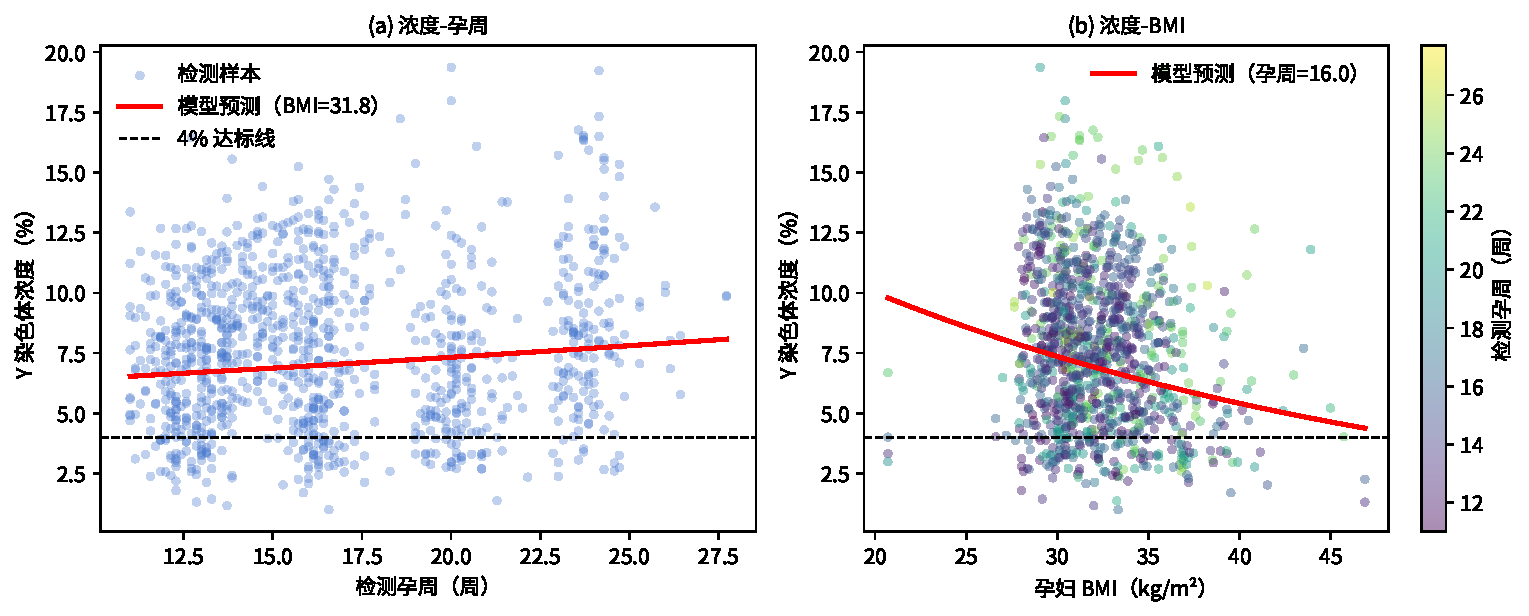
\includegraphics[width=.95\textwidth]{fig_q1_scatter.pdf}
\caption{Y 浓度与孕周、BMI 的散点及模型曲线（红色虚线为 4\% 达标线）}\label{fig:q1scatter}
\end{figure}
\begin{figure}[H]\centering
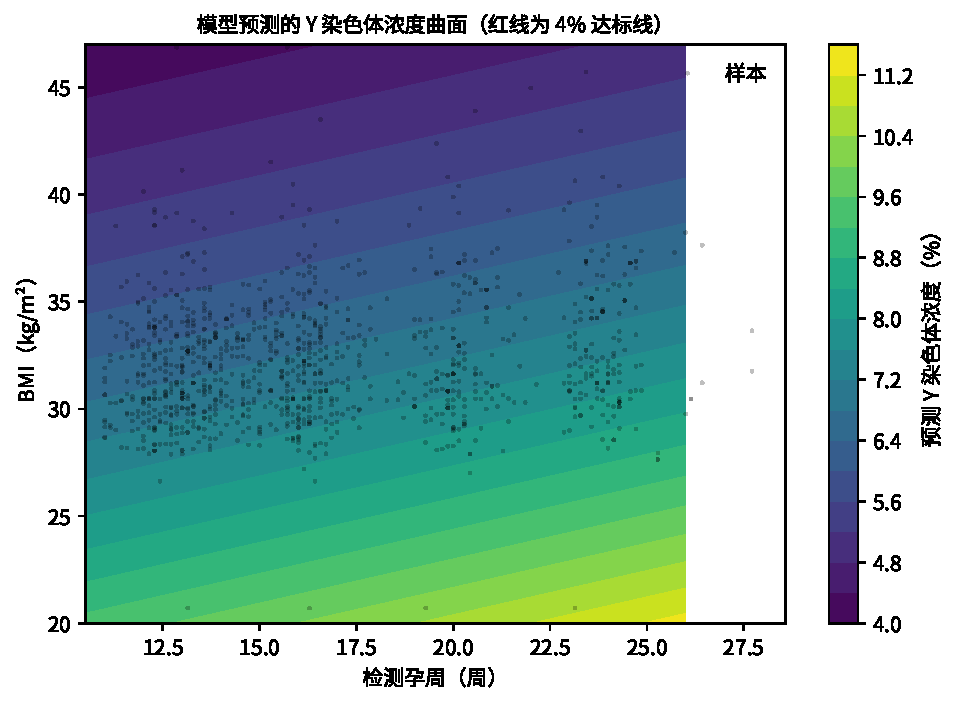
\includegraphics[width=.72\textwidth]{fig_q1_surface.pdf}
\caption{模型预测的 Y 浓度曲面与 4\% 达标等值线（红）}\label{fig:q1surf}
\end{figure}

\section{问题2：BMI 分组与最佳 NIPT 时点}
\subsection{达标概率的验证}
对 BMI 组 $\times$ 孕周段统计经验达标比例，与模型 $\Phi\big((\mu(t,b)-\ln0.04)/s\big)$ 对照（$s^2=\tau^2+\sigma^2=0.220$），22 个有效格子中模型与经验值平均偏差约 4 个百分点（例如 $[10,12)$ 周 $\times$ BMI$[28,32)$：经验 0.886 vs 模型 0.871；$[12,14)\times[32,36)$：0.888 vs 0.847），可用于时点优化。

\subsection{期望风险递推与分组优化}
给定首次检测时点 $t_0$，有效概率 $p_{\rm valid}(t,b)=(1-p_{\rm fail}(t))\,\Phi((\mu(t,b)-\ln0.04)/s)$；无效则 $\delta$ 周后复查，期望风险反向递推：
\begin{equation}\label{eq:risk}
R(t)=p_{\rm valid}(t)\,w(t)+\big(1-p_{\rm valid}(t)\big)\big(\lambda+R(t+\delta)\big),\quad t\le30.
\end{equation}
以带最小样本量约束的一维动态规划在 BMI 离散格（0.5）上搜索 $K=4,5,6$ 组的最优区间划分，目标为组内共用时点下 $\sum R$ 最小。结果显示 $K=4,5,6$ 的总风险几乎相同（人均 1.0442），内部细切分（29.0/29.5）无实际意义，故合并为可执行的三组方案（表~\ref{tab:q2}）。Bootstrap（200 次聚类重抽样）显示中位切点约 29 与 38，95\% 区间 [28.5,31]、[30,39.5]，高 BMI 边界稳健。

\begin{table}[H]\centering\small
\caption{推荐的 BMI 分组、最佳时点与风险指标}\label{tab:q2}
\begin{tabular}{lcccccc}
\toprule
组别 & BMI 区间 & 样本数 & 最佳时点 $t^\ast$ & 期望风险 & 平均检测次数 & 达标率\\
\midrule
G1 & $[20.5,28.5]$ & 74 & 10.0 周 & 1.026 & 1.27 & 85.1\%\\
G2 & $(28.5,38.0]$ & 959 & 10.0 周 & 1.028 & 1.28 & 83.9\%\\
G3 & $(38.0,47.0]$ & 42 & 10.25 周 & 1.458 & 2.23 & 53.5\%\\
\bottomrule
\end{tabular}
\end{table}

结果解读：(1) 由于 10--12 周经验达标率已达 82--89\%，且复查可落在低风险带内，\textbf{最优首次检测时点被压缩到可检测窗口起点 10 周}，这与"尽早发现"的临床原则一致；题给经验五分组的人均风险 1.044 与优化方案相同，说明简单经验分组的主要缺陷不在时点而在对高 BMI 人群的识别不足。(2) G3 组风险比 G1/G2 高约 42\%、平均需 2.2 次检测、近半数在窗口内难以达标（BMI$=45$ 时模型预测 50\% 分位达标时间超出 26 周），应列为重点管理人群：10--10.5 周首检、间隔 2 周复查，两次未达标即联合侵入性诊断。经验最早达标周数（左截断下）亦显示 BMI 36--40 组中位 16.7 周、40+ 组 20.1 周，显著晚于低 BMI 组的 12.8--13.3 周，与模型一致。

\begin{figure}[H]\centering
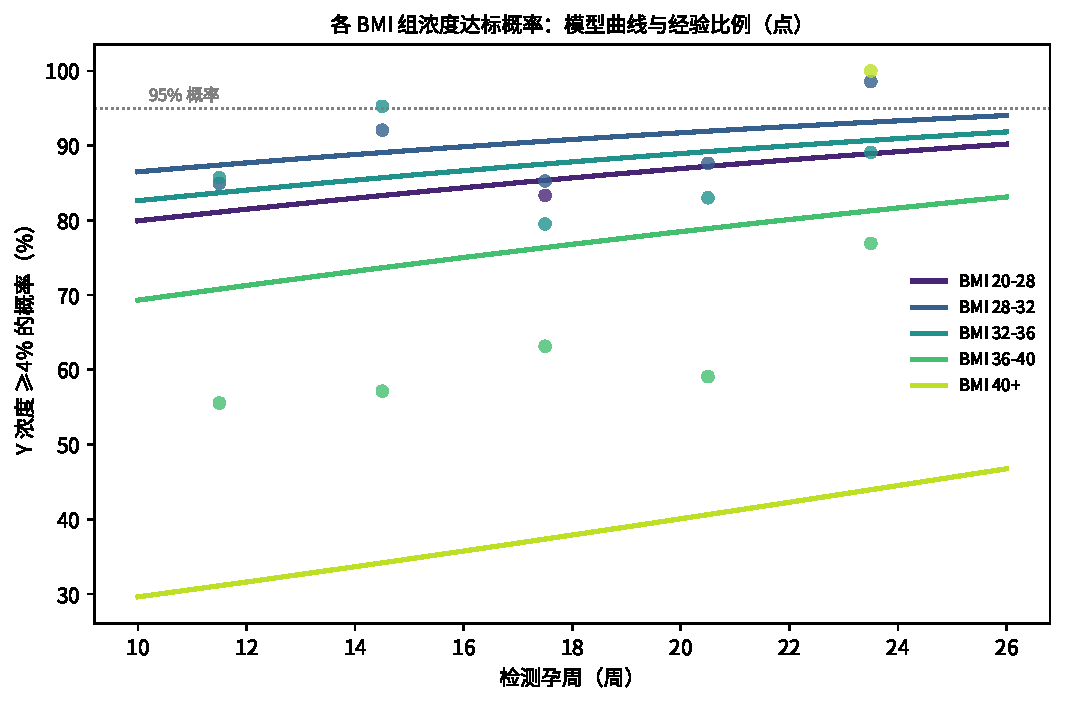
\includegraphics[width=.8\textwidth]{fig_q2_passprob.pdf}
\caption{各 BMI 组达标概率：模型曲线与经验比例（点）}\label{fig:q2pass}
\end{figure}
\begin{figure}[H]\centering
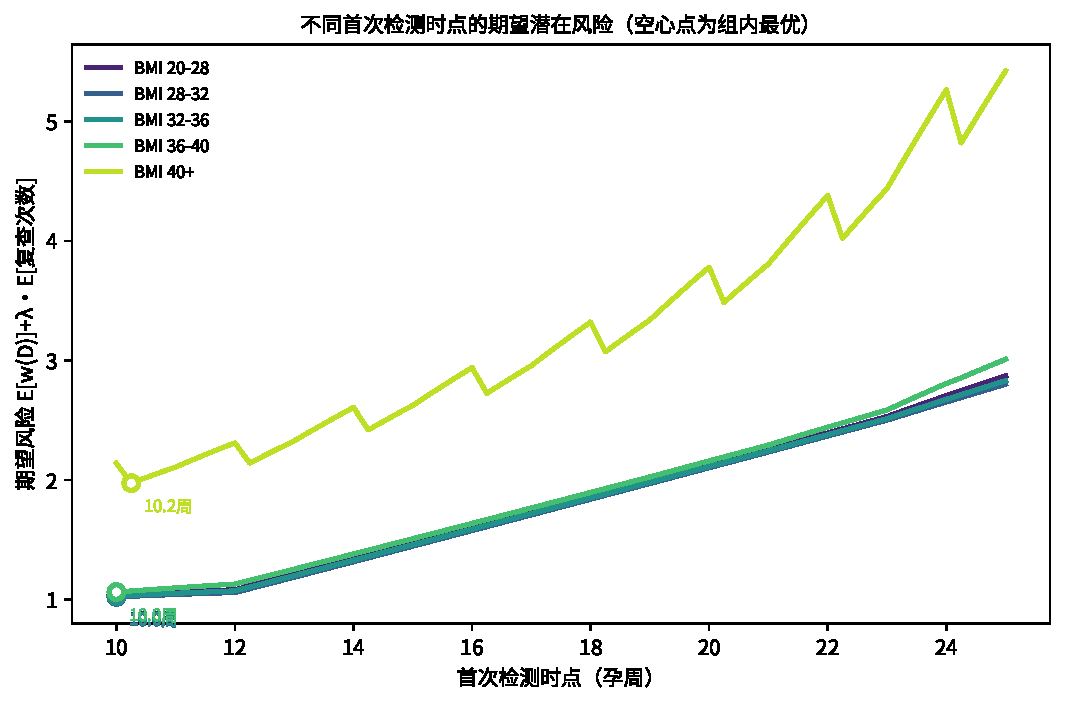
\includegraphics[width=.8\textwidth]{fig_q2_risk.pdf}
\caption{不同首次检测时点的期望风险（空心点为组内最优）}\label{fig:q2risk}
\end{figure}
\begin{figure}[H]\centering
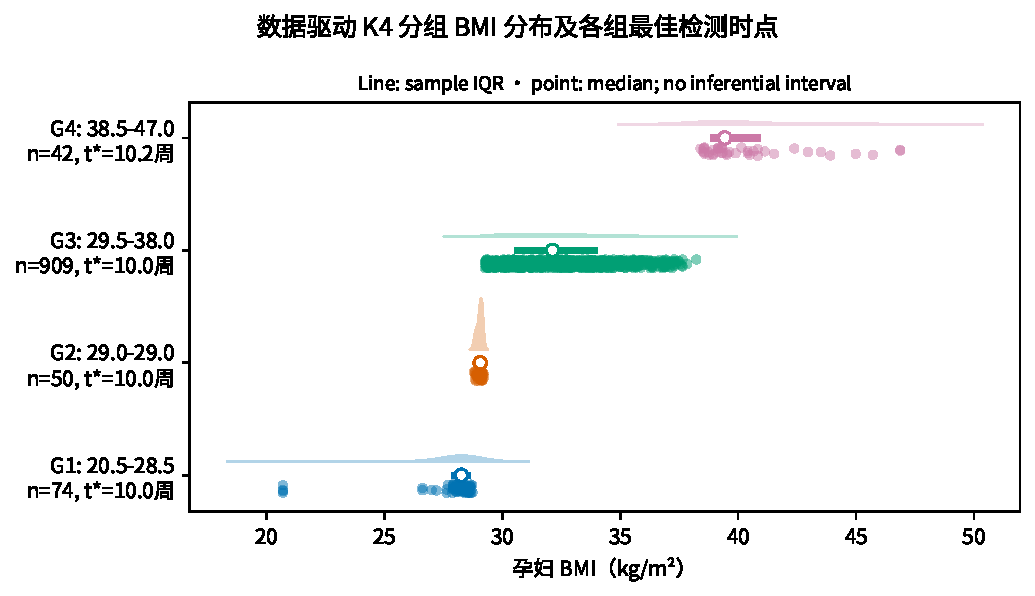
\includegraphics[width=.9\textwidth]{fig_q2_groups.pdf}
\caption{数据驱动分组的 BMI 分布与组内最佳时点}\label{fig:q2groups}
\end{figure}

\subsection{检测误差与假设的敏感性}
在浓度测量误差变异系数 0--20\% 下重算：各组最优时点不变，人均风险由 1.0442 缓升至 1.0467（+0.24\%）；测序失败早期分量 $p_{\rm early}$ 由 0 升至 0.2 时风险由 1.037 升至 1.065，时点仍不变；复查间隔 $\delta=1,2,3$ 周对应风险 1.023/1.044/1.090——\textbf{缩短复查间隔是降低高 BMI 孕妇风险最有效的杠杆}。即：检测误差主要抬高期望风险水平，而不改变"及早首检、高 BMI 加密复查"的策略（图~\ref{fig:q2err}）。

\begin{figure}[H]\centering
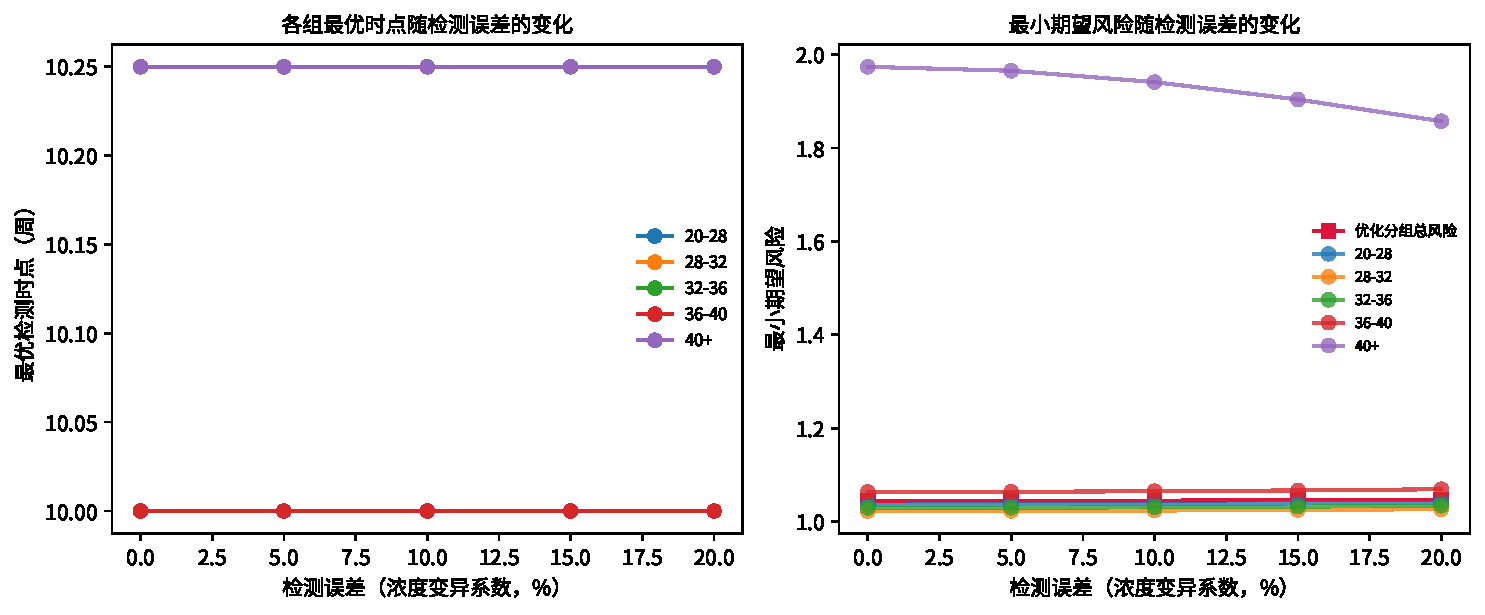
\includegraphics[width=.95\textwidth]{fig_q2_error.pdf}
\caption{检测误差敏感性：左为各组最优时点，右为最小期望风险}\label{fig:q2err}
\end{figure}

\section{问题3：综合多因素的分组与时点}
\subsection{扩展模型}
在浓度模型中引入体重 $W$、身高 $H$、年龄 $A$。统一尺度似然比较选择
\begin{equation}\label{eq:e4}
\ln C=-4.711+0.0136\,G+0.0537\,W-0.00037\,W^{2}+0.0015\,H-0.0111\,A+\varepsilon,\qquad R^{2}=0.082,
\end{equation}
其中孕周、体重（线性+二次）、年龄显著（$p=3.5\times10^{-5},\,0.020,\,0.006,\,0.003$），身高不显著（$p=0.70$）——与"母体血容量/体重稀释胎儿游离 DNA"的机制一致，身高仅提供信息而无独立效应。备选模型 E1（式(\ref{eq:m6})+年龄）中年龄同样显著（$-0.0127$，$p=9.8\times10^{-4}$）。混合效应下个体内的体重、身高、年龄效应均不显著（$p>0.13$），说明这些因素主要解释\emph{个体间}差异，而纵向变化仍由孕周主导（0.0429/周，$p\approx10^{-73}$）。

\begin{figure}[H]\centering
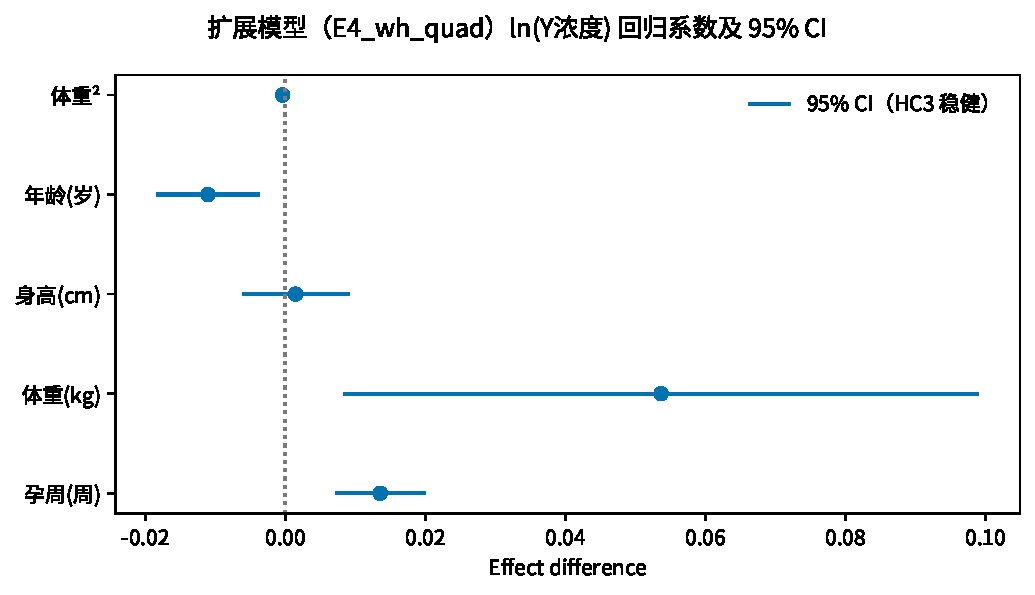
\includegraphics[width=.78\textwidth]{fig_q3_forest.pdf}
\caption{扩展模型系数及 95\% CI（标准化前）}\label{fig:q3forest}
\end{figure}

\subsection{分组、达标比例与个体化}
以扩展模型对每个个体计算风险曲线后再做动态规划，所得分组与问题2一致（人均风险 1.047 vs 1.044），各组最佳时点不变；个体化最优时点 $t_i^\ast$ 与组内统一时点几乎无差别（组内标准差 $\approx0$），即在本队列中按 BMI 三组执行统一时点不会带来可察觉的损失。达标比例：G2 组模型 83.9\%，经验（$t^\ast\pm1.5$ 周窗口，$n=18$）88.9\%；G3 组模型 56.7\%，与经验（$n=1$，参考）方向一致。误差敏感性同问题2（CV 20\% 时风险 1.050，时点不变，图~\ref{fig:q3err}）。

\begin{table}[H]\centering\small
\caption{扩展模型下的分组结果}\label{tab:q3}
\begin{tabular}{lcccccc}
\toprule
组别 & BMI 区间 & $n$ & $t^\ast$ & 期望风险 & 模型达标率 & 经验达标率\\
\midrule
G1 & [20.5,28.5] & 74 & 10.0 & 1.023 & 86.2\% & --\\
G2 & (28.5,38.0] & 959 & 10.0 & 1.029 & 83.9\% & 88.9\%\\
G3 & (38.0,47.0] & 42 & 10.25 & 1.524 & 56.7\% & --\\
\bottomrule
\end{tabular}
\end{table}

结论：纳入身高、体重、年龄后，"BMI 三组 + 窗口起点首检 + 高 BMI 加密复查"的建议保持不变；年龄与体重的作用体现在风险分层解释而非改变时点。

\begin{figure}[H]\centering
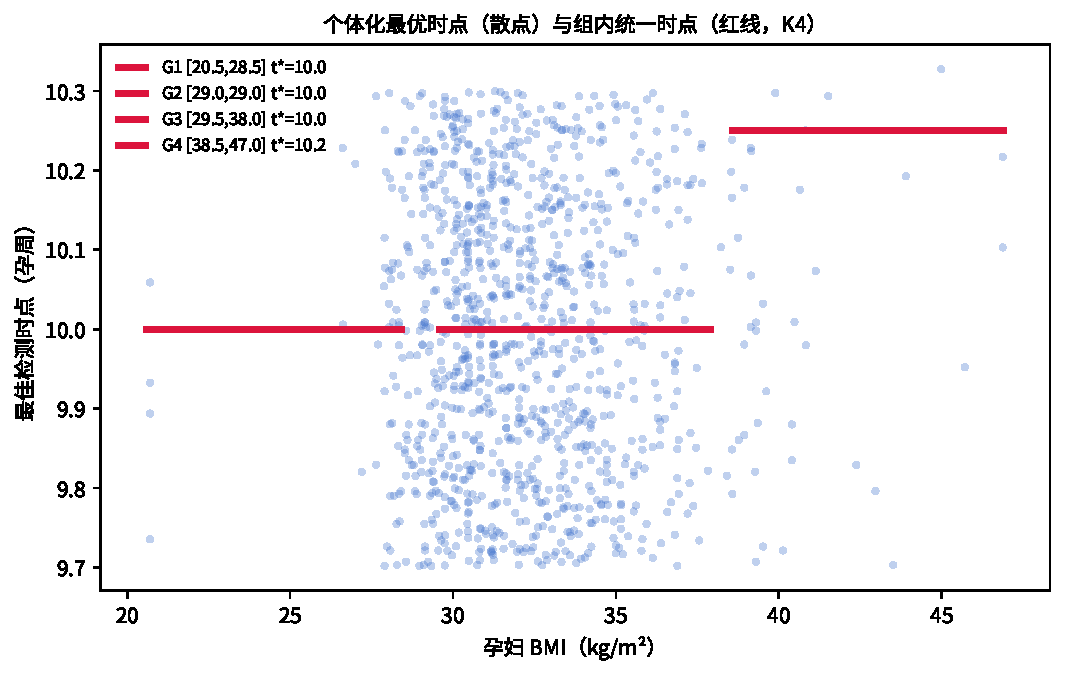
\includegraphics[width=.8\textwidth]{fig_q3_timing.pdf}
\caption{个体化最优时点（散点）与组内统一时点（红线）}\label{fig:q3timing}
\end{figure}
\begin{figure}[H]\centering
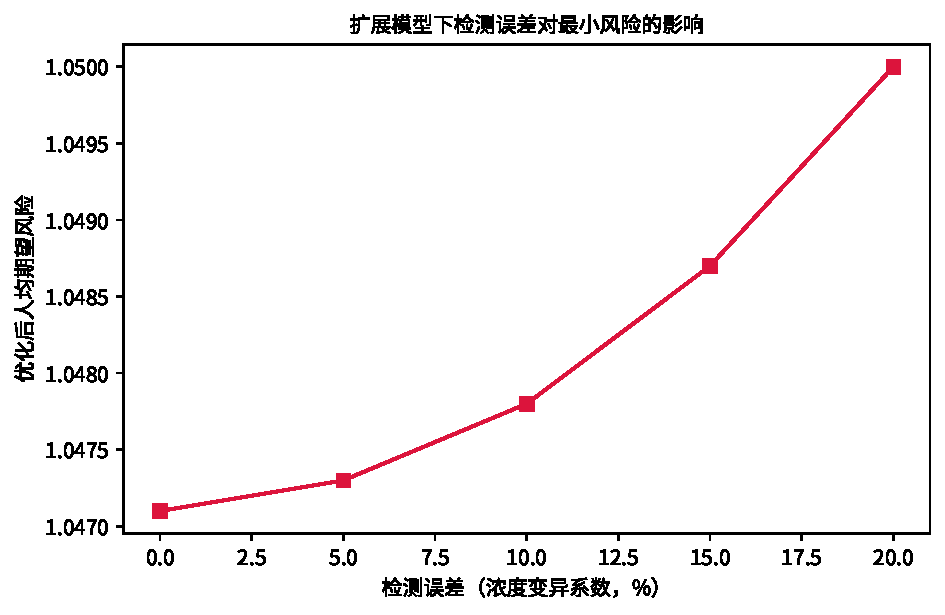
\includegraphics[width=.6\textwidth]{fig_q3_error.pdf}
\caption{扩展模型下检测误差敏感性}\label{fig:q3err}
\end{figure}

\section{问题4：女胎异常的判定方法}
\subsection{标签与基线}
以 AB 列为判定结果（67 条异常：T18 最多）。经典规则 $|Z_k|\ge3$ 的灵敏度仅 0--6\%（表~\ref{tab:q4}），因为本数据异常样本的 Z 值多数未达到 3（如 T21 异常行 $Z_{21}$ 均值 $-0.16$），单染色体阈值规则失效，必须多指标融合。

\subsection{分类模型（按孕妇分组的分层交叉验证）}
特征取 13/18/21/X 的 Z 值、X 浓度、总及各染色体 GC 含量、BMI、孕周、年龄、读段数与比对/重复/过滤比例。结果（表~\ref{tab:q4}）：对"任一异常"，logistic 回归 AUC 0.781（Youden 阈值 0.114 时灵敏度 0.687、特异度 0.768），随机森林 0.761、梯度提升 0.748；逐染色体中 T13 以随机森林最佳（AUC 0.834），T18 约 0.79；\textbf{T21 的 AUC 仅约 0.5，当前特征不含其可学习信号}，如实披露并建议该类样本送其他平台或侵入性复核。

\begin{table}[H]\centering\small
\caption{基线 $|Z|$ 规则与机器学习（分组 CV）对比}\label{tab:q4}
\begin{tabular}{lcccc}
\toprule
方法 & 目标 & AUC & 灵敏度 & 特异度\\
\midrule
$|Z|\ge3$ 规则 & 任一 & -- & 0.060 & 0.924\\
Logistic & 任一 & 0.781 & 0.687 & 0.768\\
随机森林 & T13 & 0.834 & 0.783 & 0.801\\
Logistic & T18 & 0.790 & 0.783 & 0.751\\
\bottomrule
\end{tabular}
\end{table}

\subsection{可解释判定规则}
以标准化特征拟合 logistic 得分
\begin{equation}\label{eq:q4}
s=\beta_0+\sum_k\beta_k\frac{x_k-\mu_k}{\sigma_k},\qquad P=\frac{1}{1+e^{-s}},
\end{equation}
全数据 AUC 0.861；Youden 阈值 0.166 处灵敏度 0.716、特异度 0.883（泛化性能以 CV 的 0.78 为准）。显著因素（$p<0.05$）：X 染色体浓度（$\beta=-0.92$，$p=2.5\times10^{-5}$）、21 号 GC 含量（$-4.25$，$p=5.2\times10^{-7}$）、13 号 GC 含量（$+3.32$，$p=2.2\times10^{-3}$）、X 的 Z 值（$-0.35$，$p=0.039$）、年龄（$-0.43$，$p=0.045$）、被过滤读段比例（$+0.30$，$p=0.011$）。随机森林重要性同样以 X 浓度（0.24）、13 号 GC（0.10）、BMI（0.08）居前三。生物学上：异常判定与"胎儿游离 DNA 份额偏低（X 浓度低）+ 测序/GC 分布异常"相伴，提示数据中的非整倍体标记部分源于低浓度下的测序质量扰动，判定规则据此把 Z 值、GC 含量、浓度与质量指标融合。

\textbf{建议的判定流程}：① 逐染色体计算得分 $s_k$（logistic，特征以对应 $Z_k$、GC$_k$、X 浓度为主），$P_k\ge$ 阈值判为该号染色体疑似非整倍体；② 任一 $P_k$ 超阈或综合得分 $P\ge0.17$ 判为"异常待确认"，结合 X 浓度与过滤比例评估可信度；③ 对判异常者 2 周内复查或转侵入性诊断；④ T21 因特征信号不足一律联合复核。

\begin{figure}[H]\centering
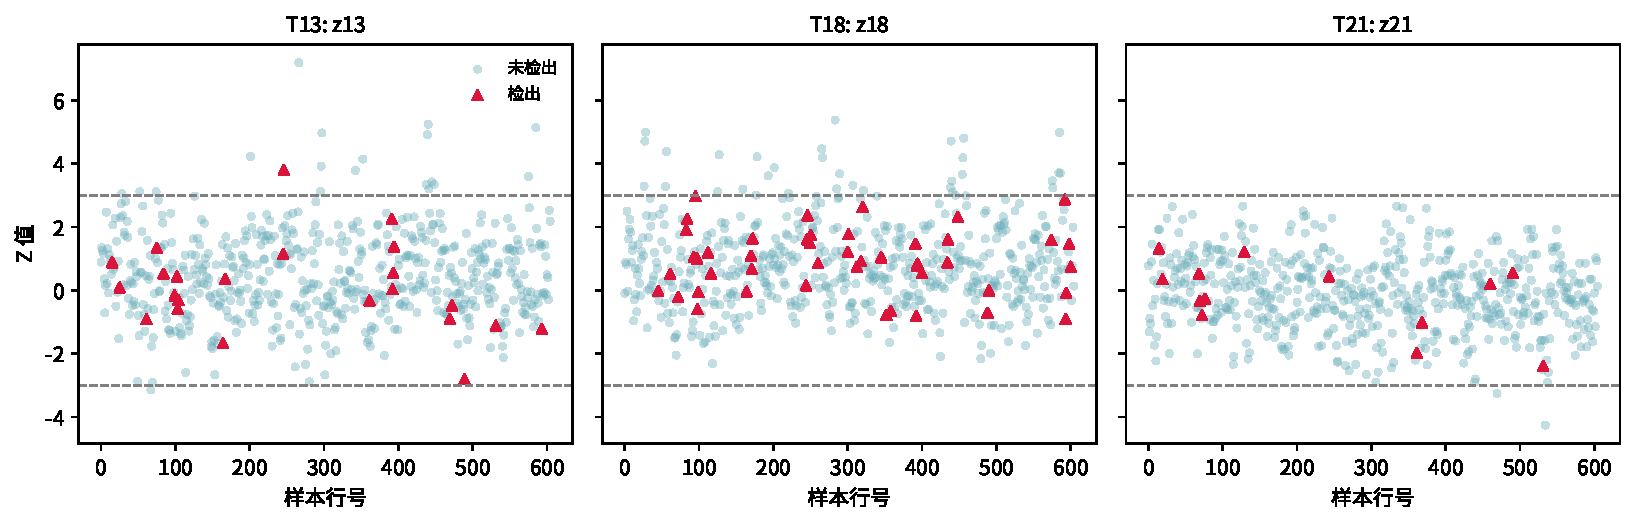
\includegraphics[width=.98\textwidth]{fig_q4_z.pdf}
\caption{13/18/21 号染色体 Z 值按标签着色：异常样本多未越出 $\pm3$ 虚线}\label{fig:q4z}
\end{figure}
\begin{figure}[H]\centering
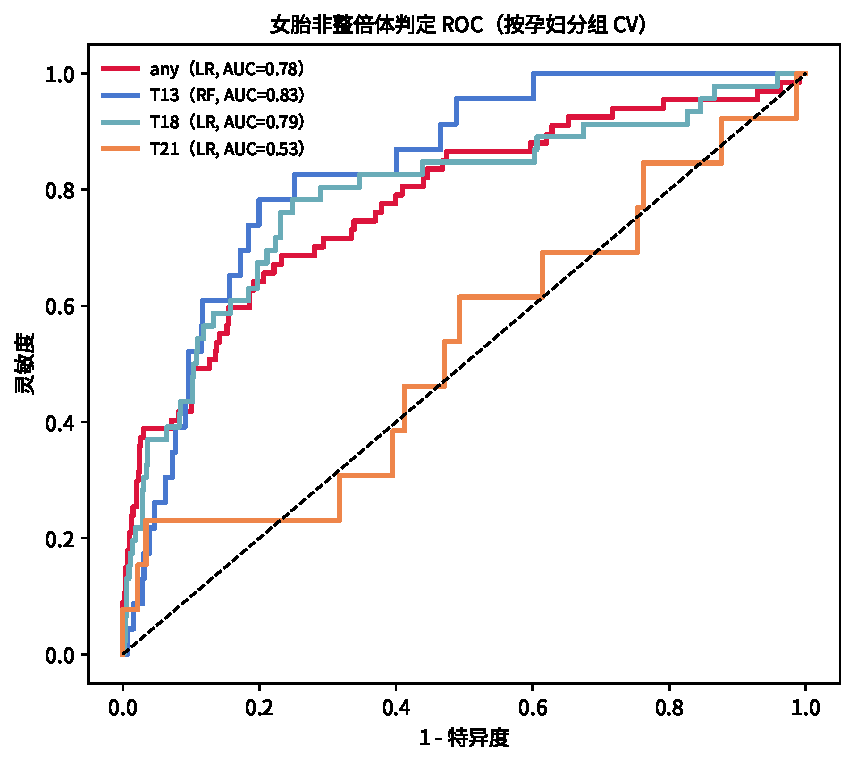
\includegraphics[width=.62\textwidth]{fig_q4_roc.pdf}
\caption{各判定目标的 ROC 曲线（按孕妇分组 CV）}\label{fig:q4roc}
\end{figure}
\begin{figure}[H]\centering
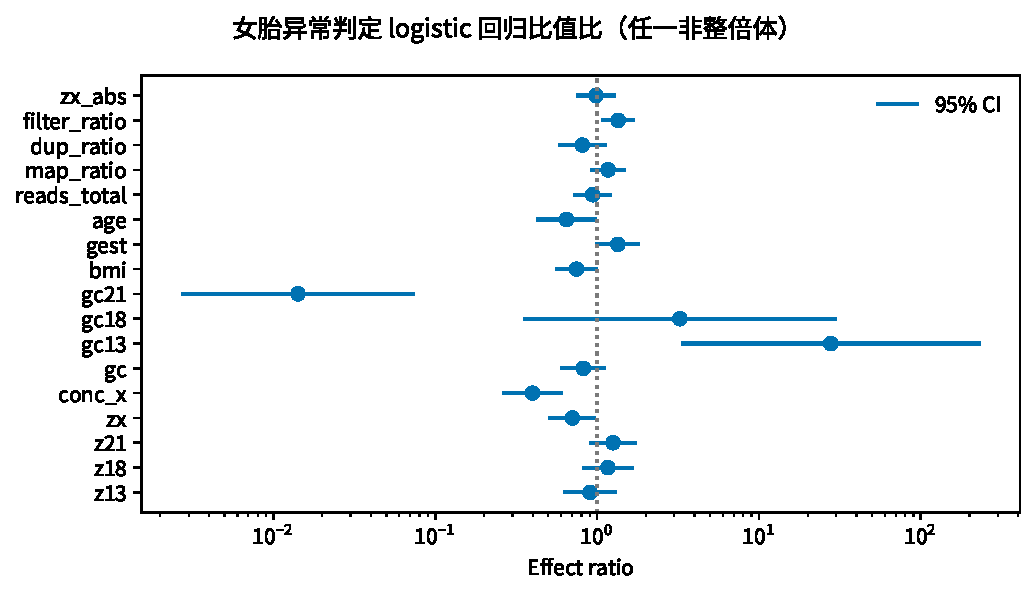
\includegraphics[width=.72\textwidth]{fig_q4_or.pdf}
\caption{综合判定 logistic 比值比（标准化特征）}\label{fig:q4or}
\end{figure}
\begin{figure}[H]\centering
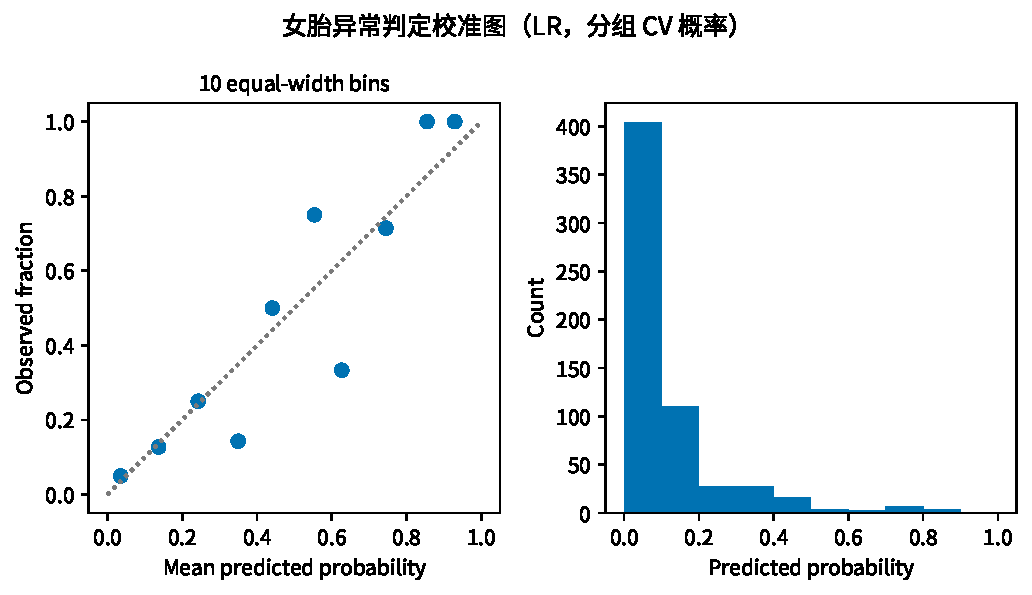
\includegraphics[width=.85\textwidth]{fig_q4_calibration.pdf}
\caption{判定概率校准图（CV 概率）}\label{fig:q4cal}
\end{figure}

\section{模型评价}
\textbf{优点}：(1) 全部推断使用稳健标准误与按孕妇分组的交叉验证，重复测量结构由混合效应显式建模；(2) 风险模型把题目定性的"低/高/极高"风险连续化并给出可复核的递推式，结论经误差、失败率、复查间隔三重敏感性验证；(3) 分组采用带最小样本量约束的动态规划并以 bootstrap 报告切点不确定性；(4) 对 T21 不可学习、标签为逐次判定等局限如实披露。
\textbf{局限}：(1) $R^2$ 较低（0.06--0.08），浓度个体差异大，时点建议应结合个体复查而非单次预测；(2) 测序失败函数与复查代价为假设参数，虽经敏感性分析仍需在真实成本下校准；(3) 女胎标签为 NIPT 自身判定且新生儿均健康，规则学习的是"检测判定"而非出生结局；(4) 10 周时点的外推依赖模型在 10--12 周的良好校准。

\section{结论}
(1) Y 浓度随孕周上升、随 BMI 先升后降（顶点约 29.6），对数线性二次模型与混合效应模型均高度显著；(2) 推荐三组方案：BMI$\le28.5$、28.5--38、$>38$，最佳首检时点分别为 10、10、10--10.5 周，高 BMI 组间隔 2 周复查、两次未达标转侵入性诊断；检测误差不改变该策略；(3) 加入体重、身高、年龄后结论稳健，年龄与体重解释个体间差异；(4) 女胎判定应采用多指标 logistic/树模型融合（AUC 0.78--0.83），摒弃单一 $|Z|\ge3$ 规则，T21 需联合复核。

\begin{thebibliography}{9}
\bibitem{rolnick2018} Rolnick N, et al. Influence of body mass index on fetal fraction increase with gestation and cell-free DNA test failure. Obstetrics \& Gynecology, 2018.
\bibitem{korean2023} Cell-Free Fetal DNA Screening Analysis in Korean Pregnant Women: Six Years of Experience. J. Pers. Med. 2023, 13(10):1468.
\bibitem{early2026} Clinical Feasibility of Early First-Trimester Non-Invasive Prenatal Testing. PubMed 42083549, 2026.
\bibitem{lo1997} Lo Y M D, et al. Presence of fetal DNA in maternal plasma and serum. Lancet, 1997.
\end{thebibliography}

\appendix
\section{可复现性声明}
全部计算使用 Python（pandas/NumPy/SciPy/statsmodels/scikit-learn），脚本位于 \texttt{work/scripts/}（q1--q4\_analysis.py 等），中间结果位于 \texttt{work/results/}，图元文件位于 \texttt{work/figures/}。分析由 AI 智能体辅助完成，图表均由数据驱动代码生成，未使用图像生成模型伪造数值。

\end{document}
